%!TEX program = lualatex
\documentclass[tikz]{standalone}
\usepackage{luatex85, shellesc}
\usetikzlibrary{}

\begin{document}
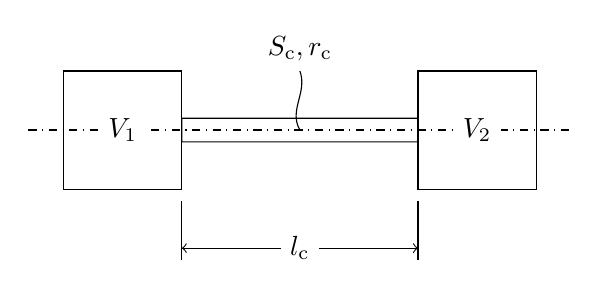
\begin{tikzpicture}[scale=1.5]
    %\draw[style=help lines] (0,0) grid (13,6);
  \draw [dashdotted] (-0.3,0) -- (4.3,0);
  \draw (0,-0.5)rectangle (1,0.5) node [midway,fill=white] {$V_1$};
  \draw [shift={(1,0)}] (0,-0.1) rectangle (2,0.1)
                        (1,0) to[out=120,in=-70] (1,0.5) node [above] {$S_\mathrm{c}, r_\mathrm{c}$};
  \draw [shift={(3,0)}] (0,-0.5) rectangle (1,0.5) node [midway,fill=white] {$V_2$};
  \draw [shift={(1,-0.5)}, <->] (0,-0.1) -- (0,-0.6)
                                (2,-0.1) -- (2,-0.6)
                                (0,-0.5) -- (2,-0.5) node [midway,fill=white] {$l_\mathrm{c}$};
  
\end{tikzpicture}
\end{document}